\begin{frame}
  \frametitle{Modello di Sverdrup (1953)}
  \begin{columns}

    \column{.5\textwidth}
    Penetrazione dell'intensità luminosa:    
    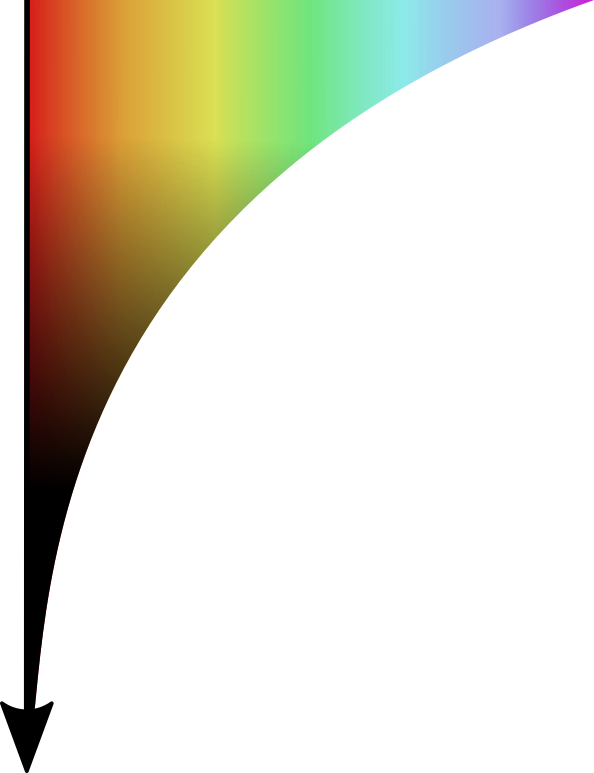
\includegraphics[width=0.7\textwidth]{../img/light_penetration}

    \column{.5\textwidth}
    Alta turbolenza
    Profondità critica per il mixed layer
    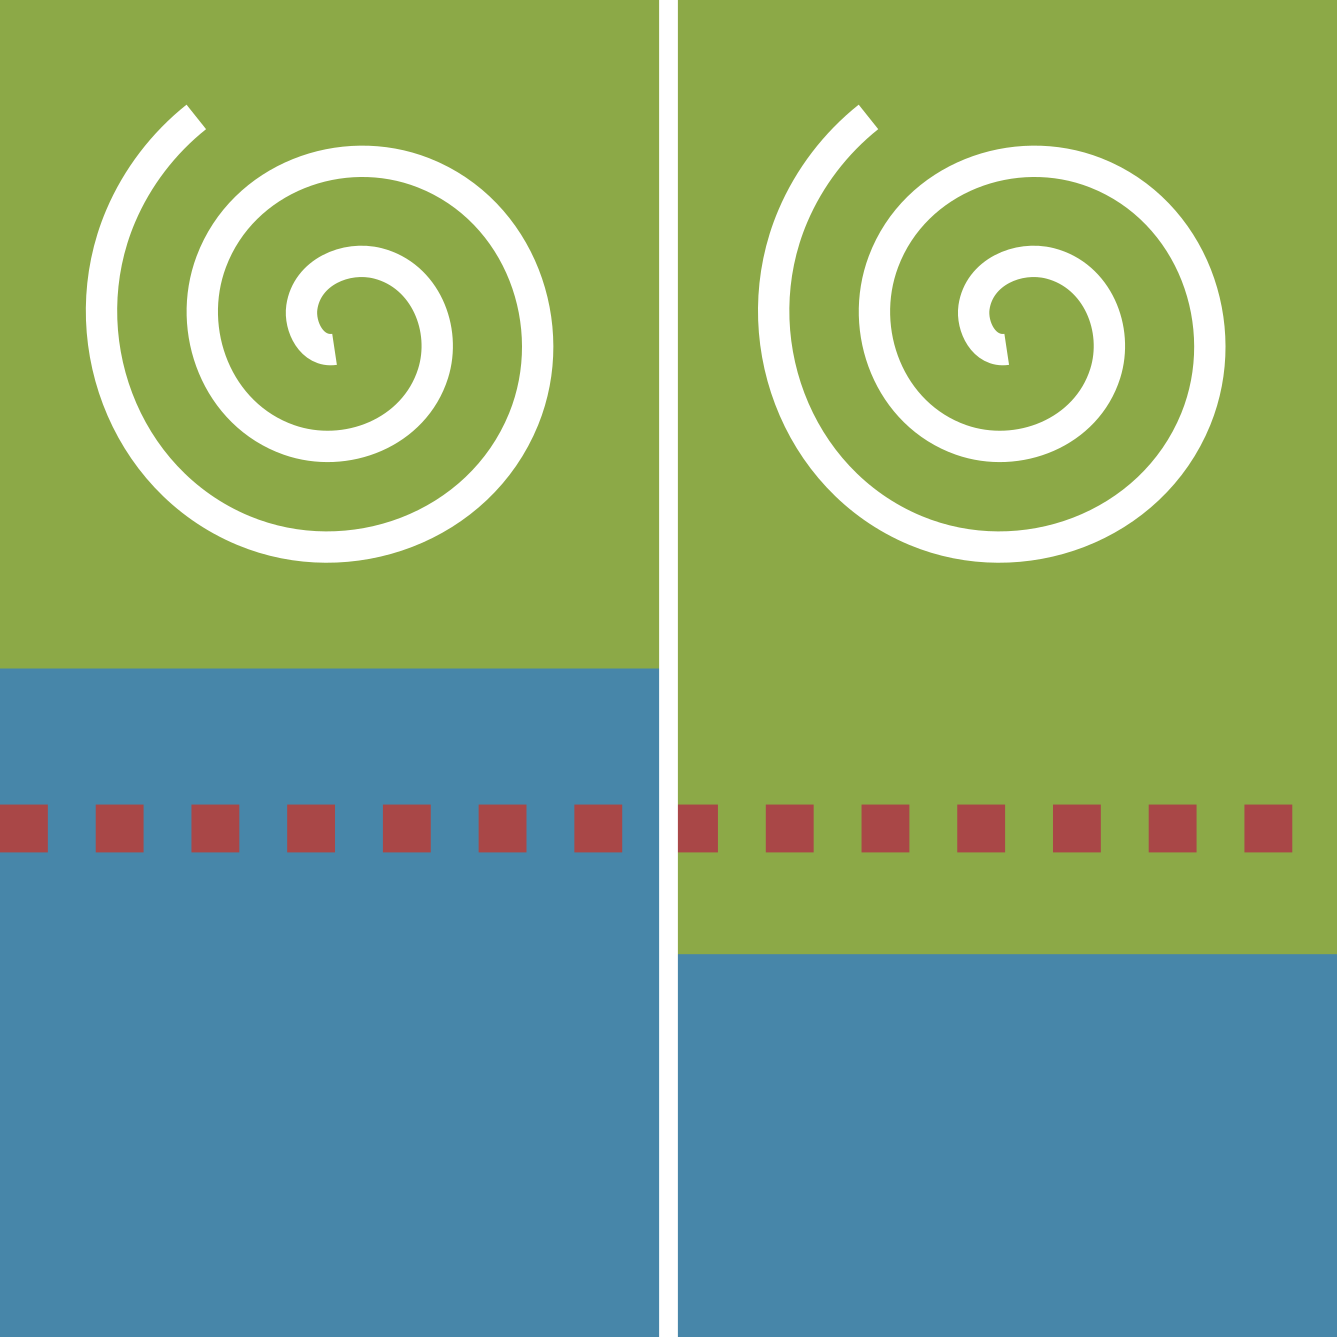
\includegraphics[width=\textwidth]{../img/critical_depth}

  \end{columns}
\end{frame}

\begin{frame}
  \frametitle{Modello di Sverdrup (1953)}
  \begin{columns}

    \column{.5\textwidth}
 Termoclina e mixed layer
    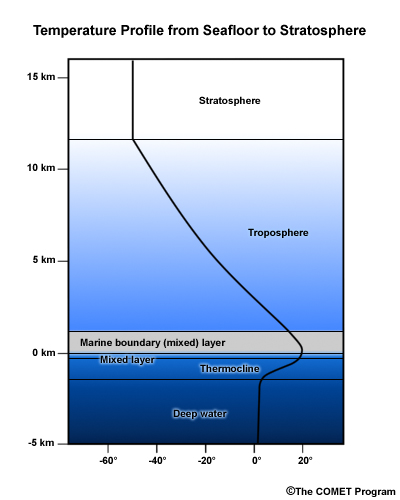
\includegraphics[width=0.7\textwidth]{../img/temp_profile}

    \column{.5\textwidth}
    Risultati
    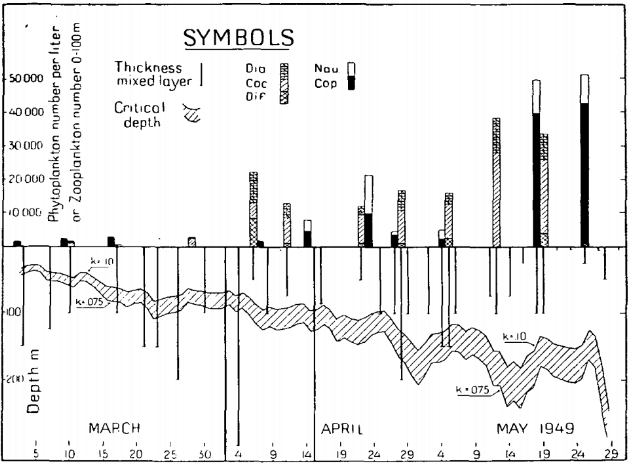
\includegraphics[width=\textwidth]{../img/Sverdrup_result}

  \end{columns}
\end{frame}
\begin{frame}
  \frametitle{Modello di Sverdrup (1953)}
  Formula per la profondità critica:
  \[ \mathrm{crescita \; netta} = \int_0^{z_c} \int_0^T (\lambda I_0(t) e^{kx} - \mu )\mathrm{d}t \mathrm{d}x \equiv 0 \]
  \[ \frac{z_c}{e^{kz_c}-1} =-\frac{\lambda}{\mu}\frac{\bar{I}}{k} \]

\end{frame}

\begin{frame}
  \frametitle{Modello Shigesada-Okubo (1981)}
  \[ n(z,t) \]
  \[ \partial_t n + v \partial_z n = D \partial_z^2 n + (g(z,n) - \mu) n \]
  \[ g(z,n) =  \lambda \frac{I(z,t)}{I(z,t)+h} \]
  \[ I(z,t) = e^{-k_{bg} z - k_{as}\int_0^z n(z,t) \mathrm{d}z } \]

\end{frame}

\begin{frame}
  \frametitle{Condizioni al contorno}

  \begin{columns}
    \column{0.5\textwidth}
    Riflettenti 
    \begin{figure}
      
\includegraphics[width=.7\textwidth]{../img/noML}
    \end{figure}

    \column{0.5\textwidth}
    Assorbenti
    \begin{figure}
      
\includegraphics[width=.7\textwidth]{../img/ML}
    \end{figure}

  \end{columns}
\end{frame}


\begin{frame}
  \frametitle{Modello di Huisman (2002)}
  \begin{columns}

    \column{.5\textwidth}
    \includegraphics<1>[width=\textwidth]{../img/result_Huis_lowvel}
    \includegraphics<2>[width=\textwidth]{../img/result_Huis_hivel}
    \\
    (Huisman 2002)

    \column{.5\textwidth}
    \begin{itemize}
      \item Huisman, 1999: ipotesi della turbolenza critica; 2002: modello numerico
      \item parametri: profondità, turbolenza, velocità di affondamento
      \item profondità di compensazione: crescita locale netta nulla
      \item \( D_{min} \propto v^2 \)
    \end{itemize}

  \end{columns}
\end{frame}

\begin{frame}
  \frametitle{Altri approcci numerici}
  \begin{columns}

    \column{.7\textwidth}
    Taylor, Ferrari, 2011: LES, correlazione con flusso di calore.
    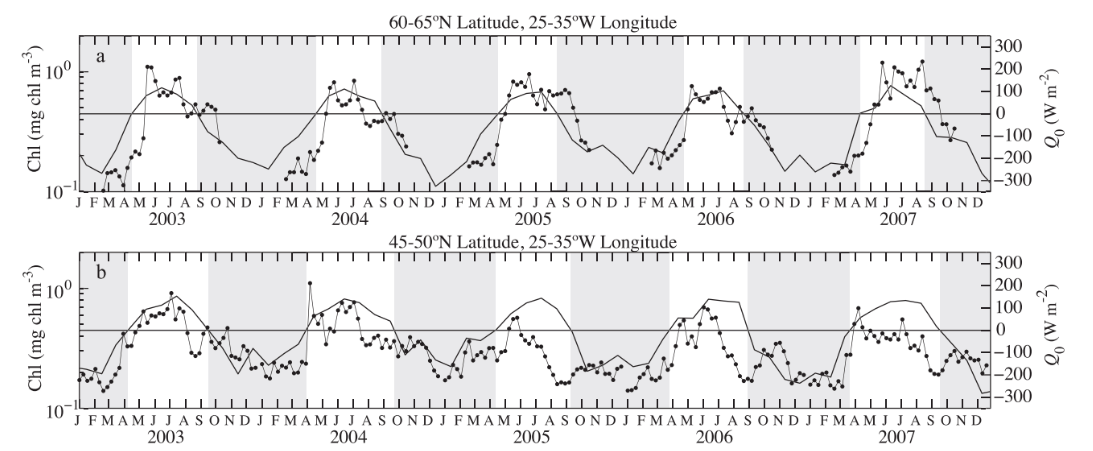
\includegraphics[width=\textwidth]{../img/Taylor2011}

    \column{.3\textwidth}
    Lindemann, Visser et al., 2017: campo di velocità imposto, deviazioni da Huisman.
    \\
    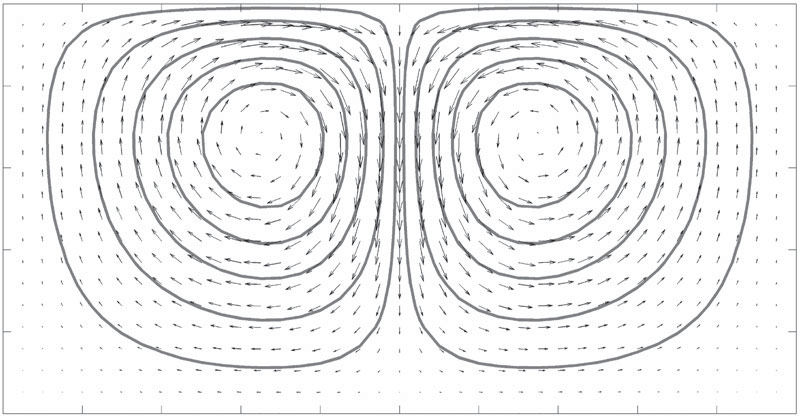
\includegraphics[width=\textwidth]{../img/Lindemann_flux}

  \end{columns}
\end{frame}


